\let\negmedspace\undefined
\let\negthickspace\undefined
\documentclass[journal]{IEEEtran}
\usepackage[a5paper, margin=10mm, onecolumn]{geometry}
\usepackage{lmodern} % Ensure lmodern is loaded for pdflatex
\usepackage{tfrupee} % Include tfrupee package

\setlength{\headheight}{1cm} % Set the height of the header box
\setlength{\headsep}{0mm}     % Set the distance between the header box and the top of the text

\usepackage{gvv-book}
\usepackage{gvv}
\usepackage{cite}
\usepackage{amsmath,amssymb,amsfonts,amsthm}
\usepackage{algorithmic}
\usepackage{graphicx}
\graphicspath{{./figs/}}
\usepackage{textcomp}
\usepackage{xcolor}
\usepackage{txfonts}
\usepackage{listings}
\usepackage{enumitem}
\usepackage{mathtools}
\usepackage{gensymb}
\usepackage{comment}
\usepackage[breaklinks=true]{hyperref}
\usepackage{tkz-euclide} 
\usepackage{listings}
\usepackage{gvv}                                        
\def\inputGnumericTable{}                    
\usepackage[latin1]{inputenc}                                
\usepackage{color}                                            
\usepackage{array}                                            
\usepackage{longtable}                                       
\usepackage{calc}                            
\usepackage{multirow}                                         
\usepackage{hhline}                                          
\usepackage{ifthen}                                           
\usepackage{lscape}
\usepackage{circuitikz}

\begin{document}
	
	\bibliographystyle{IEEEtran}
	\vspace{3cm}
	
	\title{4.7.39}
	\author{EE25BTECH11042 - Nipun Dasari}
	\maketitle
	
	\renewcommand{\thefigure}{\theenumi}
	\renewcommand{\thetable}{\theenumi}
	\setlength{\intextsep}{10pt} % Space between text and floats
	
	
	\numberwithin{equation}{enumi}
	\numberwithin{figure}{enumi}
	\renewcommand{\thetable}{\theenumi}
	
	\textbf{Question}:\\
	The distance of the point P(2, 3) from the x-axis is?  \\ 
	
	\solution \\
	
	Let the position vector of the point P(2, 3) be represented as $\vec{p}$. :
	\begin{align}
		\vec{p} = \begin{myvec}{ 2 \\ 3 }\end{myvec}
	\end{align}
	

	Consider the general line equation where 
	\begin{align}
		\vec{n}^\top\vec{x} = c
	\end{align}
	Using the fact that all y-coordinates of x axis are zero

	\begin{align}
		 \vec{n} = \begin{myvec} { 0\\ 1} \end{myvec} \text{ and } c=0 \label{1}
	\end{align}
	
	The distance between a $\vec{p}$ to its foot of perpendicular to a line is: 
	\begin{align}
		\text{Distance} = \frac{|\vec{n}^\top\vec{p}-c|}{\norm{\vec{n}}} \label{2}
	\end{align}
	By \eqref{2} and \eqref{1}:
	\begin{align}
		\text{Distance} = \frac{|\begin{myvec} { 0& 1} \end{myvec}\begin{myvec}{ 2 \\ 3 }\end{myvec}-0|}{1}\\
		= 2\times0 + 3\times1 = 3
	\end{align}
	Therefore, the distance of point P from the x-axis is $3$ units.
	
	\begin{figure}[H]
		\centering
		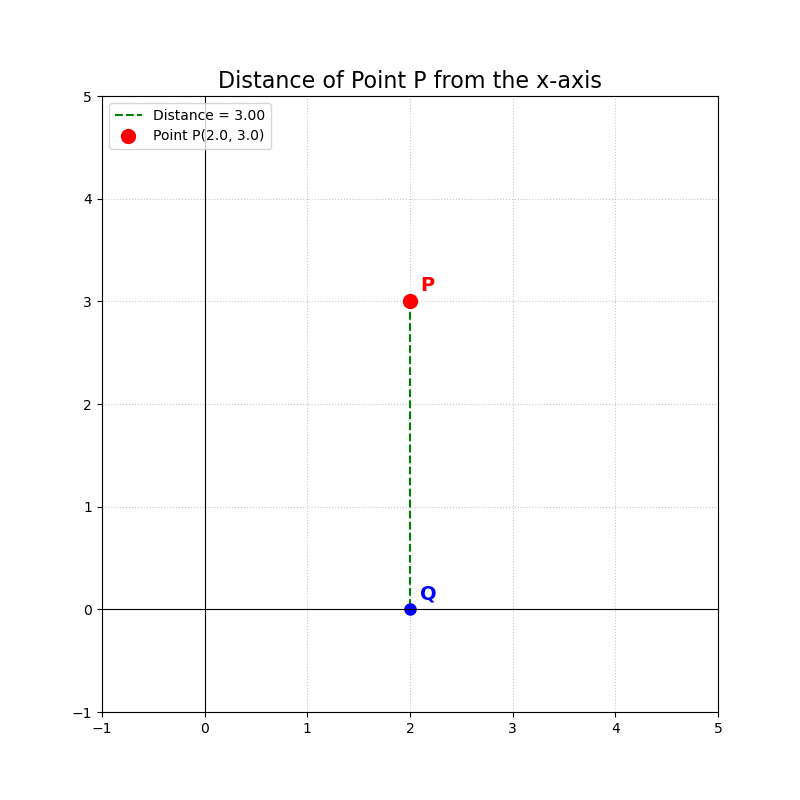
\includegraphics[width = 0.8\columnwidth]{Figure_1.png}
		\caption*{}
		\label{fig_dist}
	\end{figure}
	
\end{document}